In this section, three factors, including the frame length of the sliding window, the angle of the movement, and the number of radars are investigated in micro-Doppler based classification. It is helpful to assess the influence of these factors on micro-Doppler data processing and model optimization, and make the micro-Doppler based human activity analysis more practical.
\begin{figure*}[!ht]
         \centering
         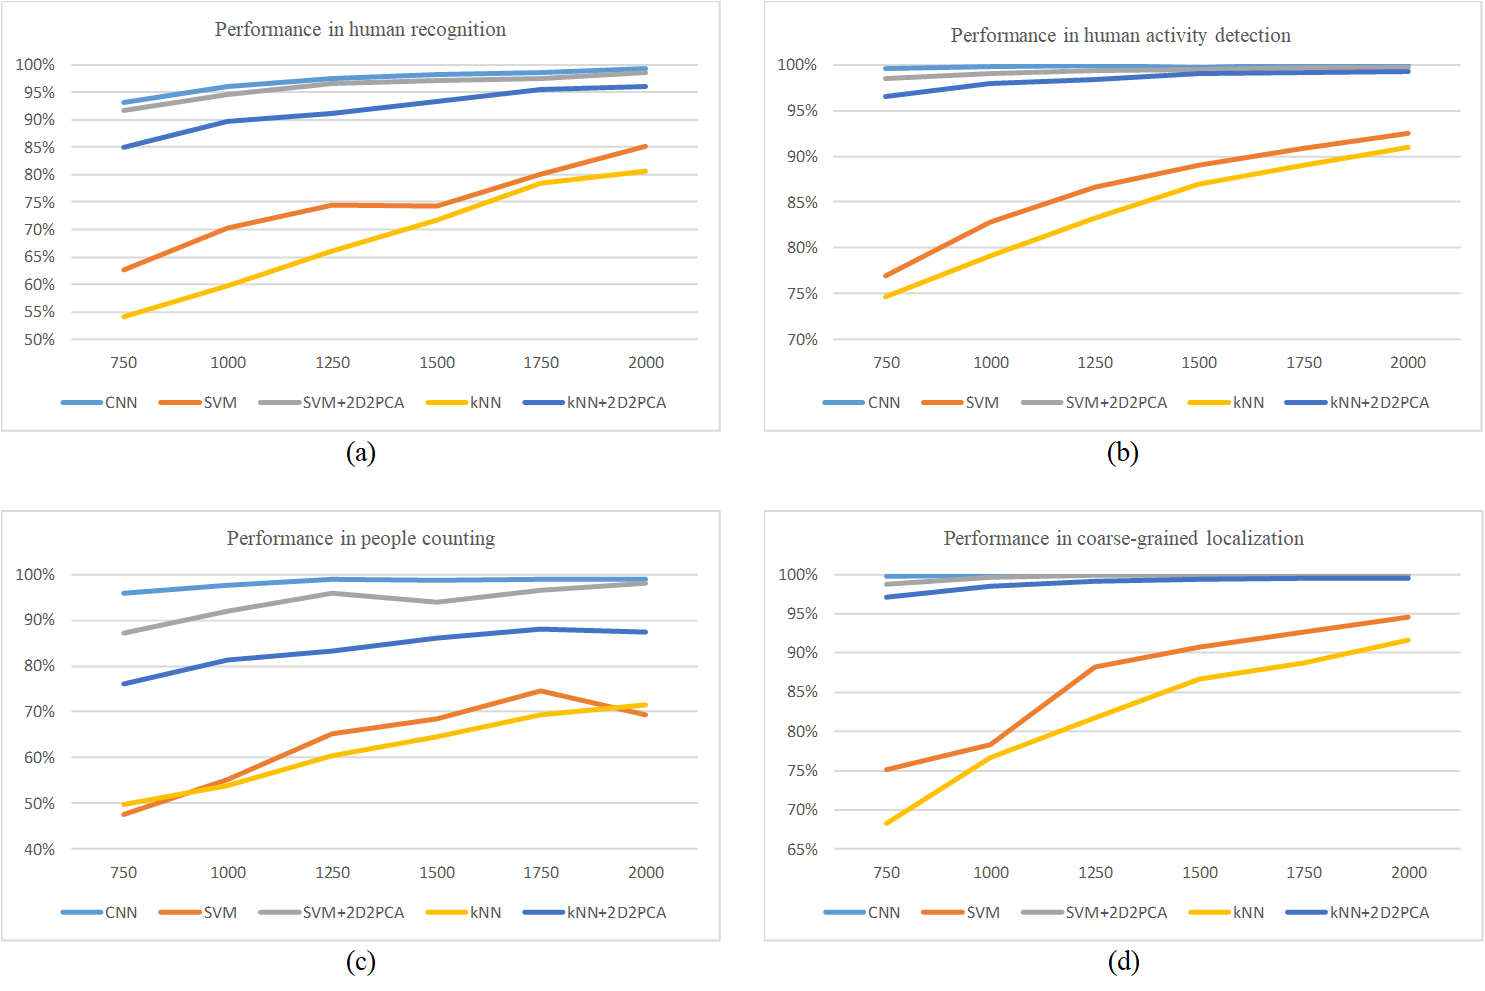
\includegraphics[width=6.8in]{frames}
         \caption{Performances (OA) of the classifiers with the changing frame lengths}
         \label{fig_frames}
\end{figure*}
\subsection{The frame length of the sliding window}
As mentioned in Section IV, the radar signals are processed with STFT, which uses a sliding window with a given frame length to generate spectrograms. It is worth studying how the different frame lengths affect the classification. 

Six frame lengths, including 750 samples, 1000 samples, 1250 samples, 1500 samples, 1750 samples, and 2000 samples are investigated here. As the sample frequency is 250 Hz, the frame length also can be measured in the time domain. Then the six frame lengths also can be measured as 3s, 4s, 5s, 6s, 7s, and 8s. With the generated samples, the classifiers are used to perform the classification. As shown in Fig. \ref{fig_frames}, the performances (OA used) of almost all classifiers increase with the increasing frame length for all four classification tasks. Although the amount of the increase declines for greater frame lengths. The superiority of the classifier’s performance remains the same as stated in section VII, which is still $CNN>(SVM+2D2PCA)>(kNN+2D2PCA)>SVM>kNN$. Therefore, it is plausible to conclude that increasing the frame length of the sliding window can increase the classification accuracy. A longer frame length means the sliding window contains more information that makes the classification easier. In reality, it is not possible to increase the frame length endlessly, because each activity has a time period. Also, a longer frame length means a longer sampling time interval that results in higher latency, which delays the classification results. So, the frame length is determined based on the tradeoff between the classification accuracy and the latency. The frame length used in this research was 5s, which led to good accuracies and low latency. Also, the time of 5s was a suitable period to measure the movement in detection area, because the walking or the running along the detection area usually took 4-7s.

\subsection{Angles of the movement}
In Section III, we stated that the experiments were made from three different angles ($\ang{0}$, $\ang{45}$, and $\ang{90}$). The coarse-grained localization made in \textit{Case 3} was investigated from two angles ($\ang{45}$ and $\ang{90}$). As shown in Fig. \ref{fig_angles}, the classifications for human activity detection and people counting performed best with samples from $\ang{0}$ that reached 100\% and 99.46\% overall accuracies for the respective classification tasks. Samples from \ang{45} produced the worst results, which were 99.7\% and 97.7\% in human activity detection and people counting respectively. For the coarse-grained localization, the same OA (100\%) was achieved at both \ang{45} and \ang{90}. It means the angle of the movements has little effect to the classification accuracy in localization. In conclusion, the direction of the movement to the radar beam can affect the classification in human activity and people counting, and \ang{0} can provide the best accuracy, followed by \ang{90} and \ang{45}. This is probably because the RCS is largest when people move at \ang{0}.  While for the coarse-grained localization, the angle of movement direction had no practical effect.
\begin{figure}[!ht]
         \centering
         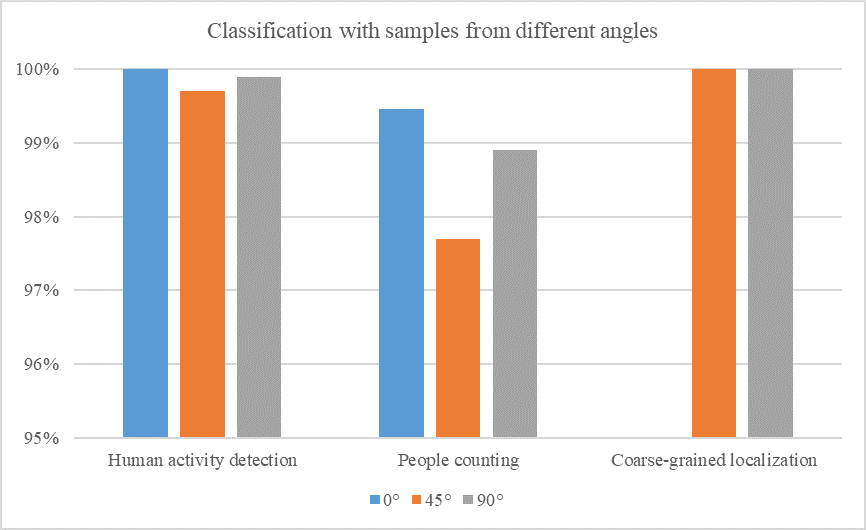
\includegraphics[width=3.5in]{angles}
         \caption{Performances of the classifiers in the tasks with the changing frame lengths}
         \label{fig_angles}
\end{figure}
\subsection{Number of Doppler Radars}
The radar system built in this research consisted of two radars. In the data processing, the signals from both radars were fused together. In this section, we investigate how the number of radars affects the classification results. For this purpose, a new CNN model 'RadarNet\textsubscript{new}' was trained using only the data from the primary radar node. 
\begin{table}[]
\centering
\caption{Structure of RadarNet and RadarNet\textsubscript{new}}
\label{tb-srr}
\begin{tabular}{|c|c|}
\hline
\textbf{RadarNet} & \textbf{RadarNet\textsubscript{new}} \\ \hline
X ($50\times 50\times 2$)       & X ($50\times50\times1$)          \\ \hline
Conv1-16@$48\times48\times1$  & Conv1-12@$48\times48\times1$     \\ \hline
maxpool           & Maxpool              \\ \hline
BN                & BN                   \\ \hline
Conv2-32@$22\times22\times1$  & Conv2-24@$22\times22\times1$     \\ \hline
maxpool           & Maxpool              \\ \hline
BN                & BN                   \\ \hline
Dropout (0.3)     & Dropout (0.3)        \\ \hline
Conv3-48@$9\times9\times1$    & Conv3-24@$9\times9\times1$       \\ \hline
Flatten           & Flatten              \\ \hline
BN                & BN                   \\ \hline
Dropout (0.4)     & Dropout (0.4)        \\ \hline
FCL-350           & FCL-256              \\ \hline
BN                & BN                   \\ \hline
Dropout (0.3)     & Dropout (0.3)        \\ \hline
FCL-160           & FCL-76               \\ \hline
\multicolumn{2}{|c|}{FCL (Softmax)}      \\ \hline
\end{tabular}
\end{table}

The main difference between RadarNet\textsubscript{new} and RadarNet is the input size, which is $50\times 50\times 1$ for RadarNet\textsubscript{new}, and $50\times 50\times 2$ for RadarNet. Because one radar generates one spectrogram at each time step, the shape of each spectrogram is $50\times 50\times 1$. As seen in Table \ref{tb-srr}, the structure of both CNNs are very similar, both contain 3 convolutional layers, 2 max-pooling layers, and 2 fully connected layers. However, RadarNet\textsubscript{new} presents less feature maps and hidden units. The comparison of their performances is shown in Fig. \ref{fig_radars}. As it can be noted, the performance obtained from two radars is higher than the performance obtained by using only one radar in all four classification tasks. For human activity detection and coarse-grained localization, the results presented by the CNN using data from one radar were slightly inferior to those of using data from two radars. While in human recognition, and especially in people counting, the overall accuracy scores obtained by the data from two radars exceeded those from one radar by a large margin. In people counting, the overall accuracy score with one radar data was 91.57\%, while for two radar data it reached 98.85\%. In human recognition, the overall accuracy with one radar was 95.70\%, while the one with two radars reached 97.5\%. It is plausible to conclude that increasing the number of radars the accuracy of micro-Doppler based classification also increases. However, this increase is very small to human activity detection and coarse-grained localization, but very obvious to human recognition and people counting.
\begin{figure}[!ht]
         \centering
         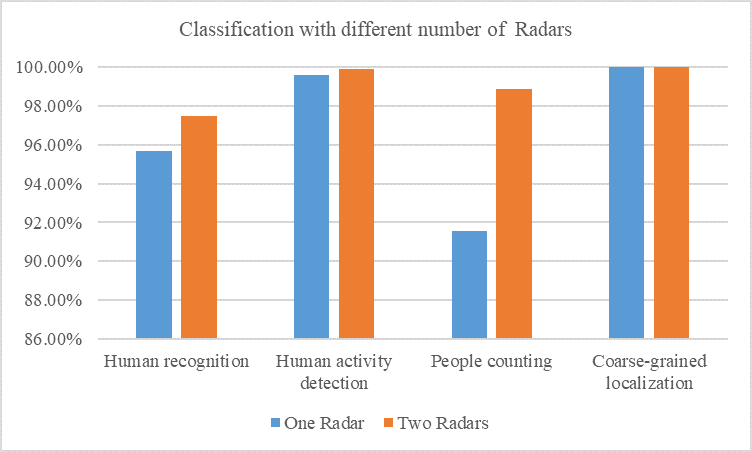
\includegraphics[width=3.5in]{radars}
         \caption{CNN classification with samples of different number of radars}
         \label{fig_radars}
\end{figure}